

\tikzset{every picture/.style={line width=0.75pt}} %set default line width to 0.75pt        

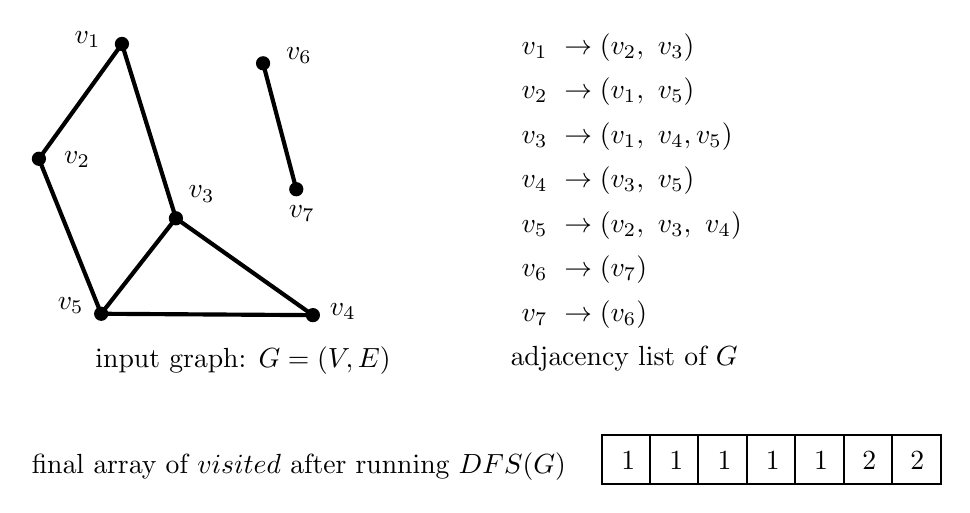
\begin{tikzpicture}[x=0.5pt,y=0.5pt,yscale=-1,xscale=1]
%uncomment if require: \path (0,353); %set diagram left start at 0, and has height of 353

%Flowchart: Connector [id:dp8937679142558405] 
\draw  [fill={rgb, 255:red, 0; green, 0; blue, 0 }  ,fill opacity=1 ] (78,14) .. controls (78,11.58) and (79.96,9.62) .. (82.38,9.62) .. controls (84.79,9.62) and (86.75,11.58) .. (86.75,14) .. controls (86.75,16.42) and (84.79,18.38) .. (82.38,18.38) .. controls (79.96,18.38) and (78,16.42) .. (78,14) -- cycle ;
%Flowchart: Connector [id:dp784072905480598] 
\draw  [fill={rgb, 255:red, 0; green, 0; blue, 0 }  ,fill opacity=1 ] (180,28) .. controls (180,25.58) and (181.96,23.62) .. (184.38,23.62) .. controls (186.79,23.62) and (188.75,25.58) .. (188.75,28) .. controls (188.75,30.42) and (186.79,32.38) .. (184.38,32.38) .. controls (181.96,32.38) and (180,30.42) .. (180,28) -- cycle ;
%Flowchart: Connector [id:dp022772254721651897] 
\draw  [fill={rgb, 255:red, 0; green, 0; blue, 0 }  ,fill opacity=1 ] (63,209) .. controls (63,206.58) and (64.96,204.62) .. (67.38,204.62) .. controls (69.79,204.62) and (71.75,206.58) .. (71.75,209) .. controls (71.75,211.42) and (69.79,213.38) .. (67.38,213.38) .. controls (64.96,213.38) and (63,211.42) .. (63,209) -- cycle ;
%Flowchart: Connector [id:dp49543195835367104] 
\draw  [fill={rgb, 255:red, 0; green, 0; blue, 0 }  ,fill opacity=1 ] (18,97) .. controls (18,94.58) and (19.96,92.62) .. (22.38,92.62) .. controls (24.79,92.62) and (26.75,94.58) .. (26.75,97) .. controls (26.75,99.42) and (24.79,101.38) .. (22.38,101.38) .. controls (19.96,101.38) and (18,99.42) .. (18,97) -- cycle ;
%Flowchart: Connector [id:dp9515784775019982] 
\draw  [fill={rgb, 255:red, 0; green, 0; blue, 0 }  ,fill opacity=1 ] (117,140) .. controls (117,137.58) and (118.96,135.62) .. (121.38,135.62) .. controls (123.79,135.62) and (125.75,137.58) .. (125.75,140) .. controls (125.75,142.42) and (123.79,144.38) .. (121.38,144.38) .. controls (118.96,144.38) and (117,142.42) .. (117,140) -- cycle ;
%Straight Lines [id:da9838237754489216] 
\draw [color={rgb, 255:red, 0; green, 0; blue, 0 }  ,draw opacity=1 ][line width=1.5]    (22.38,97) -- (82.38,14) ;
%Straight Lines [id:da9653235980831391] 
\draw [color={rgb, 255:red, 0; green, 0; blue, 0 }  ,draw opacity=1 ][line width=1.5]    (67.38,209) -- (121.38,140) ;
%Straight Lines [id:da9798242054041456] 
\draw [color={rgb, 255:red, 0; green, 0; blue, 0 }  ,draw opacity=1 ][line width=1.5]    (121.38,140) -- (82.38,14) ;
%Straight Lines [id:da7975395810717695] 
\draw [color={rgb, 255:red, 0; green, 0; blue, 0 }  ,draw opacity=1 ][line width=1.5]    (67.38,209) -- (22.38,97) ;
%Flowchart: Connector [id:dp5597560660362859] 
\draw  [fill={rgb, 255:red, 0; green, 0; blue, 0 }  ,fill opacity=1 ] (216,210) .. controls (216,207.58) and (217.96,205.62) .. (220.38,205.62) .. controls (222.79,205.62) and (224.75,207.58) .. (224.75,210) .. controls (224.75,212.42) and (222.79,214.38) .. (220.38,214.38) .. controls (217.96,214.38) and (216,212.42) .. (216,210) -- cycle ;
%Straight Lines [id:da7311433198213012] 
\draw [color={rgb, 255:red, 0; green, 0; blue, 0 }  ,draw opacity=1 ][line width=1.5]    (220.38,210) -- (121.38,140) ;
%Straight Lines [id:da36451088695440814] 
\draw [color={rgb, 255:red, 0; green, 0; blue, 0 }  ,draw opacity=1 ][line width=1.5]    (67.38,209) -- (220.38,210) ;
%Flowchart: Connector [id:dp4274826720632955] 
\draw  [fill={rgb, 255:red, 0; green, 0; blue, 0 }  ,fill opacity=1 ] (204,119) .. controls (204,116.58) and (205.96,114.62) .. (208.38,114.62) .. controls (210.79,114.62) and (212.75,116.58) .. (212.75,119) .. controls (212.75,121.42) and (210.79,123.38) .. (208.38,123.38) .. controls (205.96,123.38) and (204,121.42) .. (204,119) -- cycle ;
%Straight Lines [id:da8734113512633482] 
\draw [color={rgb, 255:red, 0; green, 0; blue, 0 }  ,draw opacity=1 ][line width=1.5]    (208.38,119) -- (184.38,28) ;
%Shape: Grid [id:dp9526360318390427] 
\draw  [draw opacity=0] (429,296.87) -- (674,296.87) -- (674,331.87) -- (429,331.87) -- cycle ; \draw   (464,296.87) -- (464,331.87)(499,296.87) -- (499,331.87)(534,296.87) -- (534,331.87)(569,296.87) -- (569,331.87)(604,296.87) -- (604,331.87)(639,296.87) -- (639,331.87) ; \draw    ; \draw   (429,296.87) -- (674,296.87) -- (674,331.87) -- (429,331.87) -- cycle ;

% Text Node
\draw (46,3) node [anchor=north west][inner sep=0.75pt]   [align=left] {$\displaystyle v_{1}$};
% Text Node
\draw (128.38,114.38) node [anchor=north west][inner sep=0.75pt]   [align=left] {$\displaystyle v_{3}$};
% Text Node
\draw (33.75,195) node [anchor=north west][inner sep=0.75pt]   [align=left] {$\displaystyle v_{5}$};
% Text Node
\draw (230.38,199.38) node [anchor=north west][inner sep=0.75pt]   [align=left] {$\displaystyle v_{4}$};
% Text Node
\draw (38.38,89.38) node [anchor=north west][inner sep=0.75pt]   [align=left] {$\displaystyle v_{2}$};
% Text Node
\draw (369,4.09) node [anchor=north west][inner sep=0.75pt]   [align=left] {$\displaystyle v_{1} \ \rightarrow ( v_{2} ,\ v_{3})$};
% Text Node
\draw (369,36.26) node [anchor=north west][inner sep=0.75pt]   [align=left] {$\displaystyle v_{2} \ \rightarrow ( v_{1} ,\ v_{5})$};
% Text Node
\draw (369,68.43) node [anchor=north west][inner sep=0.75pt]   [align=left] {$\displaystyle v_{3} \ \rightarrow ( v_{1} ,\ v_{4} ,v_{5})$};
% Text Node
\draw (369,100.6) node [anchor=north west][inner sep=0.75pt]   [align=left] {$\displaystyle v_{4} \ \rightarrow ( v_{3} ,\ v_{5})$ \ };
% Text Node
\draw (369,132.77) node [anchor=north west][inner sep=0.75pt]   [align=left] {$\displaystyle v_{5} \ \rightarrow ( v_{2} ,\ v_{3} ,\ v_{4})$};
% Text Node
\draw (198.75,14.35) node [anchor=north west][inner sep=0.75pt]   [align=left] {$\displaystyle v_{6}$};
% Text Node
\draw (200.75,128.35) node [anchor=north west][inner sep=0.75pt]   [align=left] {$\displaystyle v_{7}$};
% Text Node
\draw (369,164.94) node [anchor=north west][inner sep=0.75pt]   [align=left] {$\displaystyle v_{6} \ \rightarrow ( v_{7})$ \ };
% Text Node
\draw (369,197.09) node [anchor=north west][inner sep=0.75pt]   [align=left] {$\displaystyle v_{7} \ \rightarrow ( v_{6})$};
% Text Node
\draw (61,230.93) node [anchor=north west][inner sep=0.75pt]   [align=left] {input graph: $\displaystyle G=( V,E)$};
% Text Node
\draw (361,229.93) node [anchor=north west][inner sep=0.75pt]   [align=left] {adjacency list of $\displaystyle G$};
% Text Node
\draw (15,306.93) node [anchor=north west][inner sep=0.75pt]   [align=left] {final array of $\displaystyle visited$ after running $\displaystyle DFS( G)$};
% Text Node
\draw (441,306.37) node [anchor=north west][inner sep=0.75pt]   [align=left] {$\displaystyle 1$};
% Text Node
\draw (475.83,306.37) node [anchor=north west][inner sep=0.75pt]   [align=left] {$\displaystyle 1$};
% Text Node
\draw (510.66,306.37) node [anchor=north west][inner sep=0.75pt]   [align=left] {$\displaystyle 1$};
% Text Node
\draw (545.49,306.37) node [anchor=north west][inner sep=0.75pt]   [align=left] {$\displaystyle 1$};
% Text Node
\draw (580.32,306.37) node [anchor=north west][inner sep=0.75pt]   [align=left] {$\displaystyle 1$};
% Text Node
\draw (615.15,306.37) node [anchor=north west][inner sep=0.75pt]   [align=left] {$\displaystyle 2$};
% Text Node
\draw (650,306.37) node [anchor=north west][inner sep=0.75pt]   [align=left] {$\displaystyle 2$};


\end{tikzpicture}

